% Capítulo 4 – Ensayos y resultados

\chapter{Ensayos y resultados}
\label{Chapter4}

En este capítulo se describen los ensayos realizados y los resultados
obtenidos durante el desarrollo del sistema. En la
sección~\ref{sec:adquisicion} se detalla el proceso de adquisición de datos,
tanto de video como del rodillo inteligente, y el protocolo de prueba
diseñado. En la sección~\ref{sec:analisis} se presenta el análisis de los
datos recolectados, las decisiones metodológicas derivadas y las métricas de
calidad obtenidas.

% =============================================================================
\section{Adquisición de datos}
\label{sec:adquisicion}
% =============================================================================

El proceso de adquisición de datos comprendió dos fuentes principales: la
captura de video del ciclista y la lectura de métricas de rendimiento del
rodillo inteligente. A continuación se describe cada una.

% -----------------------------------------------------------------------------
\subsection{Captura de video}
\label{ssec:captura_video}
% -----------------------------------------------------------------------------

En una primera etapa, se utilizó una cámara USB Microsoft LifeCam HD-3000
con una resolución de 1280$\times$720 píxeles a 30 FPS. Se realizaron pruebas
de calidad de imagen y se determinó que el nivel de \textit{motion blur} era
excesivo. Para corroborar esta conclusión, se ejecutó el modelo de estimación
de pose HRNet sobre una muestra de los fotogramas capturados, y se constató
que las imágenes borrosas no eran detectadas por el modelo. Este resultado
confirmó que el \textit{motion blur} constituía un factor crítico para la
calidad del sistema.

Se evaluaron distintas configuraciones de la cámara, como la exposición
manual y el enfoque fijo, sin obtener mejoras significativas en la nitidez de
las imágenes. Se concluyó que la cámara no era capaz de registrar imágenes
nítidas bajo las condiciones de iluminación y movimiento presentes durante el
pedaleo. En la figura~\ref{fig:calidad_imagen} se muestra un ejemplo
representativo de los fotogramas obtenidos con esta cámara, junto con la
distribución del nivel de \textit{blur} medido.

% --- Figura: distribución de blur – LifeCam HD-3000 ---
\begin{figure}[H]
      \centering
      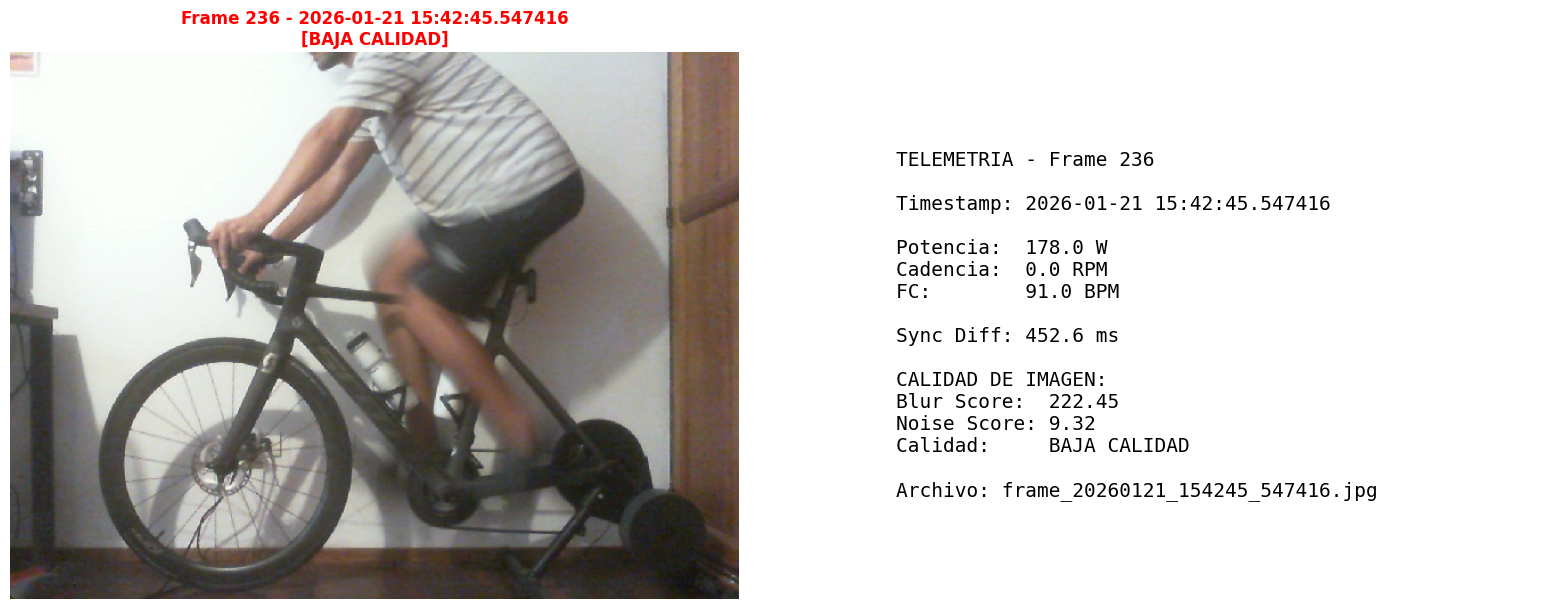
\includegraphics[width=0.80\textwidth]{./Figures/f_m_calidad.png}
      \caption{Distribución del nivel de \textit{motion blur} en las imágenes
            capturadas con la cámara Microsoft LifeCam HD-3000. El alto nivel de
            borrosidad dificultó la detección de \textit{keypoints} en las
            extremidades inferiores del ciclista.}
      \label{fig:calidad_imagen}
\end{figure}
% -------------------------------------------------------

Para resolver el problema, se adoptó el dispositivo móvil Google Pixel 8 Pro
como cámara de captura. La conexión con la computadora se estableció mediante
la aplicación DroidCam Client a través de una interfaz USB-C de alta
velocidad. En la figura~\ref{fig:calidad_pixel} se aprecia un fotograma
obtenido con esta configuración durante el pedaleo a 90~RPM; el nivel de
\textit{blur} en las extremidades inferiores del ciclista es notablemente
reducido en comparación con los fotogramas anteriores.

% --- Figura: fotograma – Google Pixel 8 Pro ---
\begin{figure}[H]
      \centering
      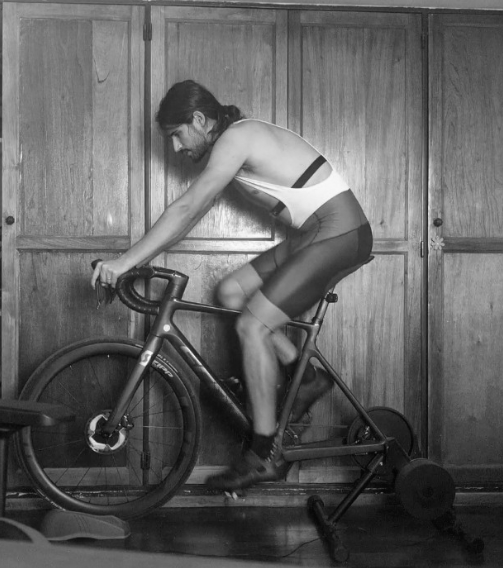
\includegraphics[width=0.80\textwidth]{./Figures/calidad_pixel8pro.png}
      \caption{Fotograma capturado con el dispositivo Google Pixel 8 Pro a
            través de DroidCam Client. El ciclista pedalea a 90~RPM y se
            aprecia un bajo nivel de \textit{motion blur} en las piernas.}
      \label{fig:calidad_pixel}
\end{figure}
% -----------------------------------------------

Se desarrolló un \textit{script} en Python para la captura y el
almacenamiento de los fotogramas. Con el fin de garantizar la trazabilidad
temporal y evitar colisiones en el sistema de archivos, los fotogramas se
nombraron con la convención \texttt{frame\_}\allowbreak%
\texttt{AAAAMMDD\_}\allowbreak\texttt{HHMMSS\_}\allowbreak%
\texttt{microsegundos.jpg},
donde \texttt{AAAAMMDD} corresponde a la fecha, \texttt{HHMMSS} a la hora y
\texttt{microsegundos} al instante de captura en microsegundos (por ejemplo,
\texttt{frame\_20260204\_224101\_848187.jpg}). El proceso de escritura en
disco se delegó a un \textit{worker} independiente, de modo que la captura no
resultara afectada por la latencia de entrada/salida.

La cámara se montó sobre un trípode a una altura de 1{,}5~m, con inclinación
nula en el eje óptico y con el plano focal perpendicular al plano de pedaleo
del ciclista. Dicha disposición permitió minimizar los efectos de perspectiva
y preparar el sistema para una eventual calibración de la cámara.

% -----------------------------------------------------------------------------
\subsection{Protocolo de prueba y datos del rodillo inteligente}
\label{ssec:protocolo_prueba}
% -----------------------------------------------------------------------------

Los datos de rendimiento del ciclista se registraron mediante un rodillo
inteligente, con la aplicación GoldenCheetah como interfaz de adquisición. La
conexión entre el rodillo y la computadora se estableció vía Bluetooth, y los
datos de potencia, cadencia y velocidad se almacenaron en formato CSV con una
resolución temporal de un segundo. La extracción de la actividad se llevó a
cabo mediante el \textit{script} \texttt{gc\_simple.py}, desarrollado con la
biblioteca \texttt{GC} de GoldenCheetah.

Se diseñó un protocolo de rampa de potencia progresiva. El ciclista comenzó
la prueba a 130~W y la carga se incrementó en escalones de 20~W cada dos
minutos hasta alcanzar los 250~W. Una vez alcanzada esa potencia, se mantuvo
durante dos minutos adicionales. Durante toda la sesión se procuró sostener
la cadencia en 90~RPM. Este diseño permitió registrar el comportamiento
biomecánico del ciclista en distintos niveles de potencia. En la
figura~\ref{fig:prueba} se muestran los datos de potencia, cadencia y
velocidad registrados durante la sesión.

% --- Figura: perfil de la prueba ---
\begin{figure}[H]
      \centering
      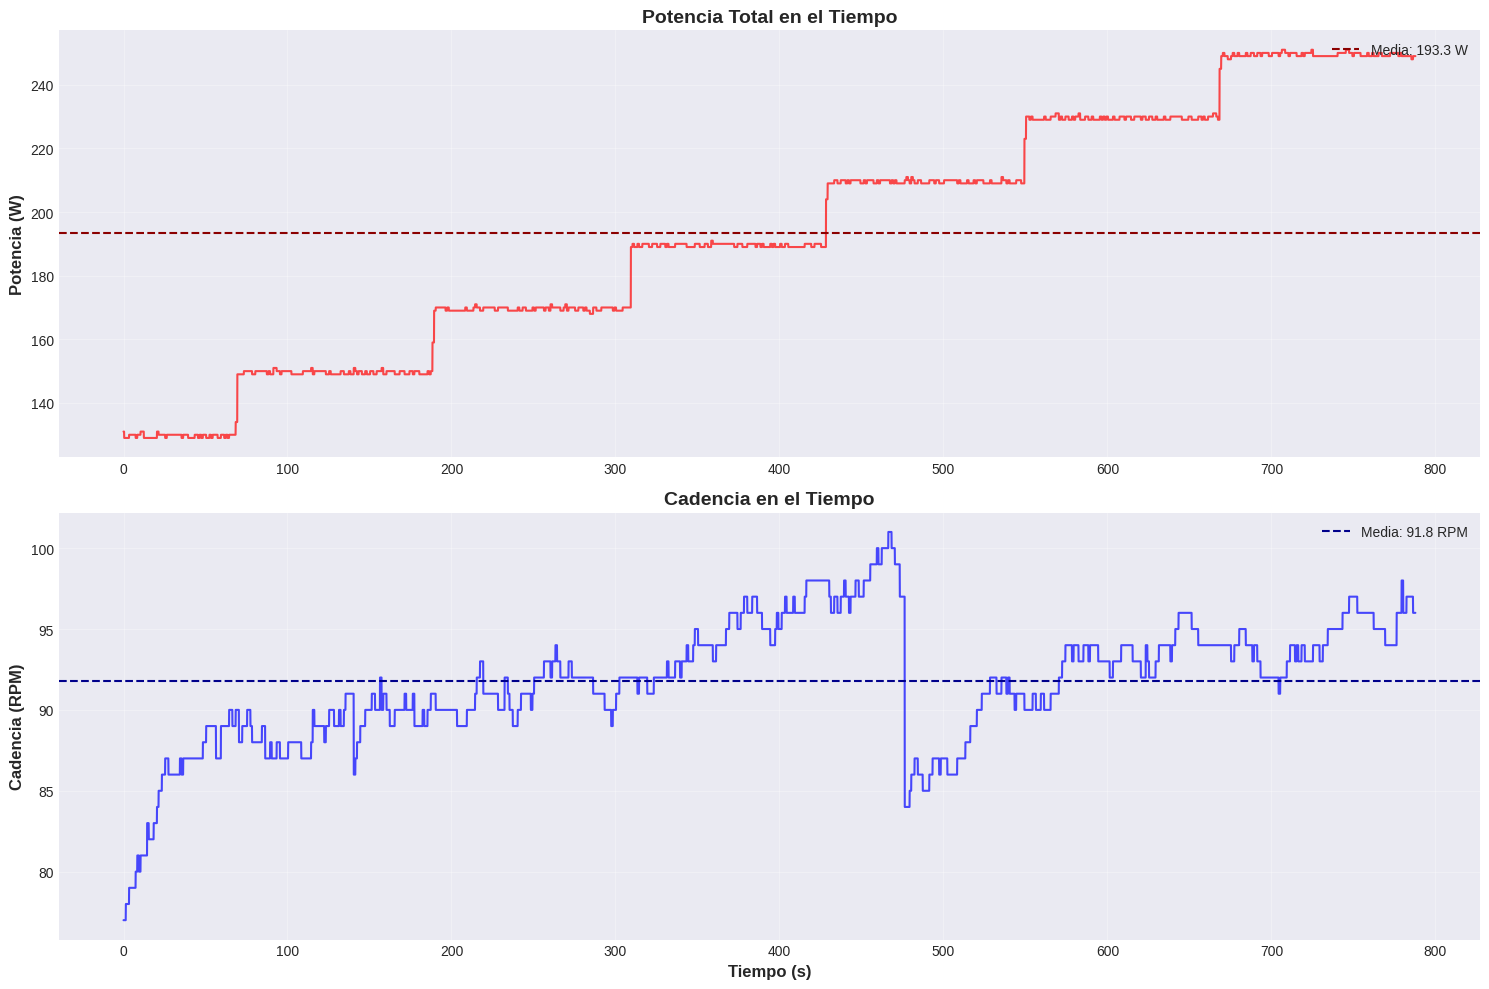
\includegraphics[width=0.85\textwidth]{./Figures/prueba_panteada.png}
      \caption{Perfil de potencia, cadencia y velocidad registrado durante el
            protocolo de rampa de potencia en el rodillo inteligente.}
      \label{fig:prueba}
\end{figure}
% ------------------------------------

Ambas fuentes de datos se activaron de forma simultánea al inicio de la
sesión para garantizar la coherencia temporal entre los fotogramas y las
métricas del rodillo.

% =============================================================================
\section{Análisis de datos}
\label{sec:analisis}
% =============================================================================

Una vez recolectados los datos, se realizó un análisis en \textit{notebooks}
de Jupyter con el objetivo de evaluar la calidad de las imágenes, caracterizar
la captura y fundamentar las decisiones metodológicas adoptadas. A
continuación se describen los análisis realizados y las decisiones derivadas.

% -----------------------------------------------------------------------------
\subsection{Calidad de imagen}
\label{ssec:calidad_imagen}
% -----------------------------------------------------------------------------

Se evaluó la nitidez de las imágenes capturadas con el dispositivo Google
Pixel 8 Pro mediante el estimador de \textit{blur} basado en el operador
laplaciano de OpenCV. El indicador se calculó sobre cada fotograma de la
sesión y se obtuvo la distribución estadística del nivel de \textit{blur}.
Los resultados confirmaron que la mayoría de las imágenes presentaban un nivel
de nitidez adecuado para la detección de \textit{keypoints}, tal como se
ilustra en la figura~\ref{fig:calidad_imagen}.

% -----------------------------------------------------------------------------
\subsection{Filtrado cinemático}
\label{ssec:filtrado_cinematico}
% -----------------------------------------------------------------------------

El análisis de la trayectoria del \textit{keypoint} correspondiente a la
rodilla indicó la presencia de valores atípicos al inicio de la sesión,
anteriores a la estabilización del ciclo de pedaleo. En la
figura~\ref{fig:trayectoria_rodilla} se aprecia este comportamiento: los
primeros fotogramas exhiben posiciones incompatibles con el patrón cíclico
del pedaleo.

% --- Figura: trayectoria de la rodilla ---
\begin{figure}[H]
      \centering
      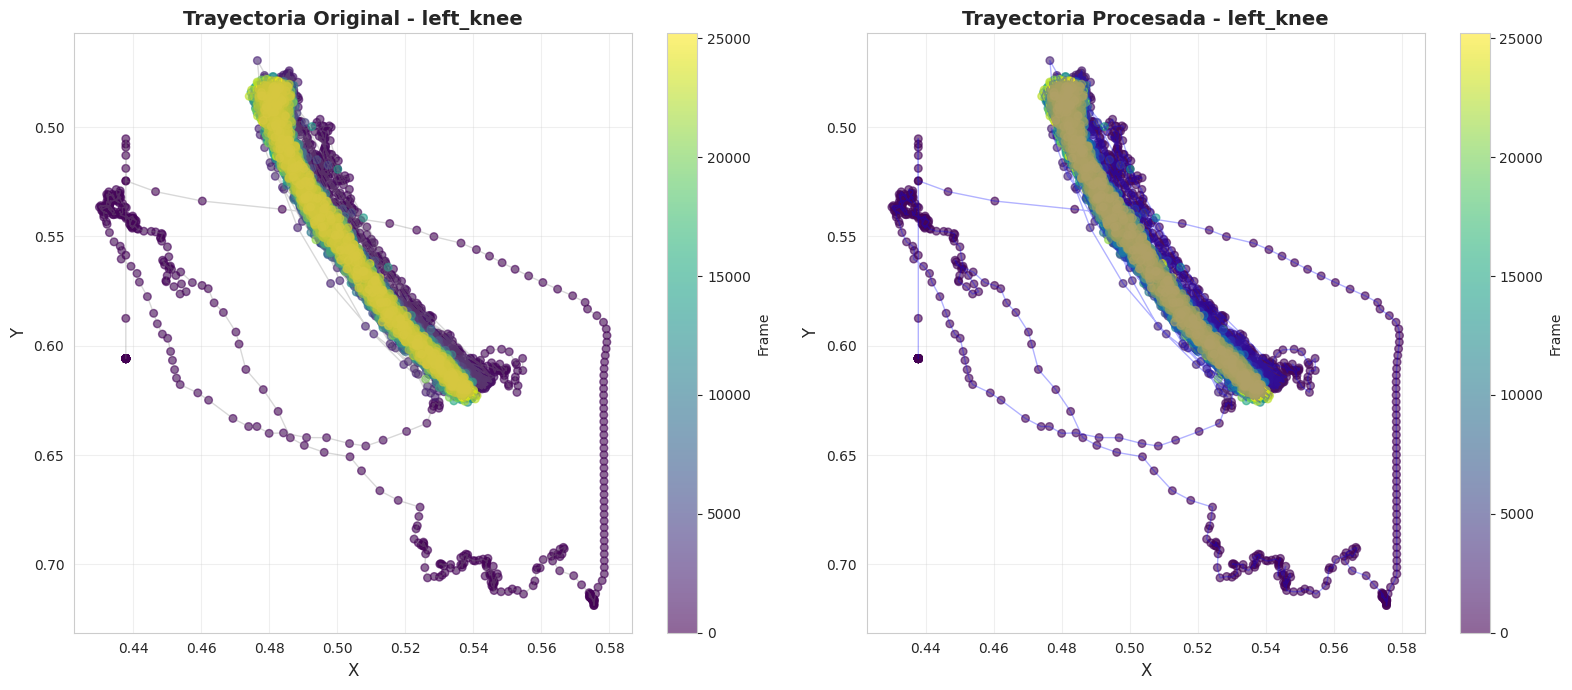
\includegraphics[width=0.80\textwidth]{./Figures/tray_rodilla.png}
      \caption{Trayectoria del \textit{keypoint} de la rodilla durante la
            sesión. Se observan valores atípicos al inicio del pedaleo,
            anteriores a la estabilización de la cadencia.}
      \label{fig:trayectoria_rodilla}
\end{figure}
% -----------------------------------------

Para mitigar este efecto, se aplicó un filtro de inicio que descarta los
fotogramas anteriores al instante en que la cadencia supera los 50~RPM de
forma sostenida. Adicionalmente, se detectó ruido en las posiciones de los
\textit{keypoints} durante el pedaleo estable, por lo que se implementó un
filtro de Kalman para el suavizado de las trayectorias. Este procedimiento
redujo los saltos discretos en la cinemática del modelo digital del ciclista
y mejoró la estabilidad del proceso de optimización de los parámetros
biomecánicos.

% -----------------------------------------------------------------------------
\subsection{Frecuencia de captura}
\label{ssec:frecuencia_captura}
% -----------------------------------------------------------------------------

Se analizó la estabilidad temporal de la captura de fotogramas a partir de
los \textit{timestamps} codificados en los nombres de archivo. En la
tabla~\ref{tab:frecuencia_captura} se resumen las estadísticas obtenidas.

% --- Tabla: frecuencia de captura ---
\begin{table}[htbp]
      \caption{Estadísticas de la frecuencia de captura de imágenes durante la
            sesión.}
      \label{tab:frecuencia_captura}
      \centering
      \small
      \begin{tabular}{lr}
            \toprule
            \textbf{Parámetro}                     & \textbf{Valor}  \\
            \midrule
            Total de fotogramas                    & 26\,155         \\
            Duración total                         & 871{,}80~s      \\
            \midrule
            Intervalo entre fotogramas mínimo      & 26{,}27~ms      \\
            Intervalo entre fotogramas máximo      & 40{,}31~ms      \\
            Intervalo entre fotogramas medio       & 33{,}33~ms      \\
            Intervalo entre fotogramas mediano     & 33{,}34~ms      \\
            \midrule
            FPS promedio                           & 30{,}00~FPS     \\
            \bottomrule
      \end{tabular}
\end{table}
% ------------------------------------

Los resultados indicaron una captura estable a 30~FPS con variación mínima en
el intervalo entre fotogramas, lo que validó el mecanismo de captura con
\textit{worker} independiente para la escritura en disco.

% -----------------------------------------------------------------------------
\subsection{Sincronización entre fuentes de datos}
\label{ssec:sincronizacion}
% -----------------------------------------------------------------------------

Dado que los datos del rodillo inteligente se registran con una resolución de
un segundo y las imágenes se capturan a 30~FPS, se cuantificó el error de
sincronización temporal entre ambas fuentes. En las
tablas~\ref{tab:resumen_sesion} y~\ref{tab:sincronizacion} se presentan el
resumen estadístico de la sesión y las métricas de sincronización obtenidas,
respectivamente.

% --- Tabla: resumen de sesión ---
\begin{table}[htbp]
      \caption{Resumen estadístico de las métricas de rendimiento registradas
            durante la sesión.}
      \label{tab:resumen_sesion}
      \centering
      \small
      \begin{tabular}{llrrrr}
            \toprule
            \textbf{Variable}  & \textbf{Unidad} & \textbf{Media} &
            \textbf{Máximo} & \textbf{Mínimo} & \textbf{Desv. est.} \\
            \midrule
            Duración total     & s    & \multicolumn{4}{c}{787{,}8}    \\
            Fotogramas         & —    & \multicolumn{4}{c}{23\,636}    \\
            Potencia           & W    & 193{,}3 & 251{,}0 & 129{,}0 & 38{,}1  \\
            Cadencia           & RPM  & 91{,}8  & 101{,}0 & 77{,}0  & 3{,}8   \\
            Frec.\ cardíaca    & BPM  & 147{,}1 & 170{,}0 & 116{,}0 & 15{,}1  \\
            \bottomrule
      \end{tabular}
\end{table}
% --------------------------------

% --- Tabla: error de sincronización ---
\begin{table}[htbp]
      \caption{Error de sincronización temporal entre la captura de imágenes y
            los datos del rodillo inteligente.}
      \label{tab:sincronizacion}
      \centering
      \small
      \begin{tabular}{lr}
            \toprule
            \textbf{Métrica}  & \textbf{Valor}   \\
            \midrule
            Error medio       & 250{,}35~ms      \\
            Error máximo      & 984{,}43~ms      \\
            \bottomrule
      \end{tabular}
\end{table}
% --------------------------------------

Con base en estos resultados, se tomaron dos decisiones metodológicas. En
primer lugar, se interpolaron los datos del rodillo inteligente para elevar
su resolución temporal a 30~FPS, de modo que cada fotograma tuviera asociada
una muestra de potencia, cadencia y velocidad. En segundo lugar, se adoptó el
\textit{timestamp} de los fotogramas como referencia temporal para la
sincronización con los datos del rodillo, dado que su resolución era superior
y correspondía al instante real de captura.

% =============================================================================
\section{\textit{Pipeline} de procesamiento y optimización}
\label{sec:pipeline}
% =============================================================================

Se diseñó un \textit{pipeline} de procesamiento que integra las dos fuentes de
datos adquiridas —video del ciclista y telemetría del rodillo inteligente— y
las transforma progresivamente hasta obtener los parámetros biomecánicos
optimizados. Las etapas que lo componen son: pasos previos de calibración y
selección de inicio, extracción de \textit{keypoints} mediante MediaPipe
BlazePose, filtrado cinemático con el filtro de Kalman, interpolación de la
telemetría a 30~FPS, construcción del modelo biomecánico digital y optimización
multiobjetivo con el algoritmo genético. En la
figura~\ref{fig:pipeline} se presenta un diagrama con la arquitectura completa
del \textit{pipeline} y el flujo de transformación de los datos a lo largo de
cada etapa.

% --- Figura: diagrama del pipeline ---
\begin{figure}[H]
      \centering
      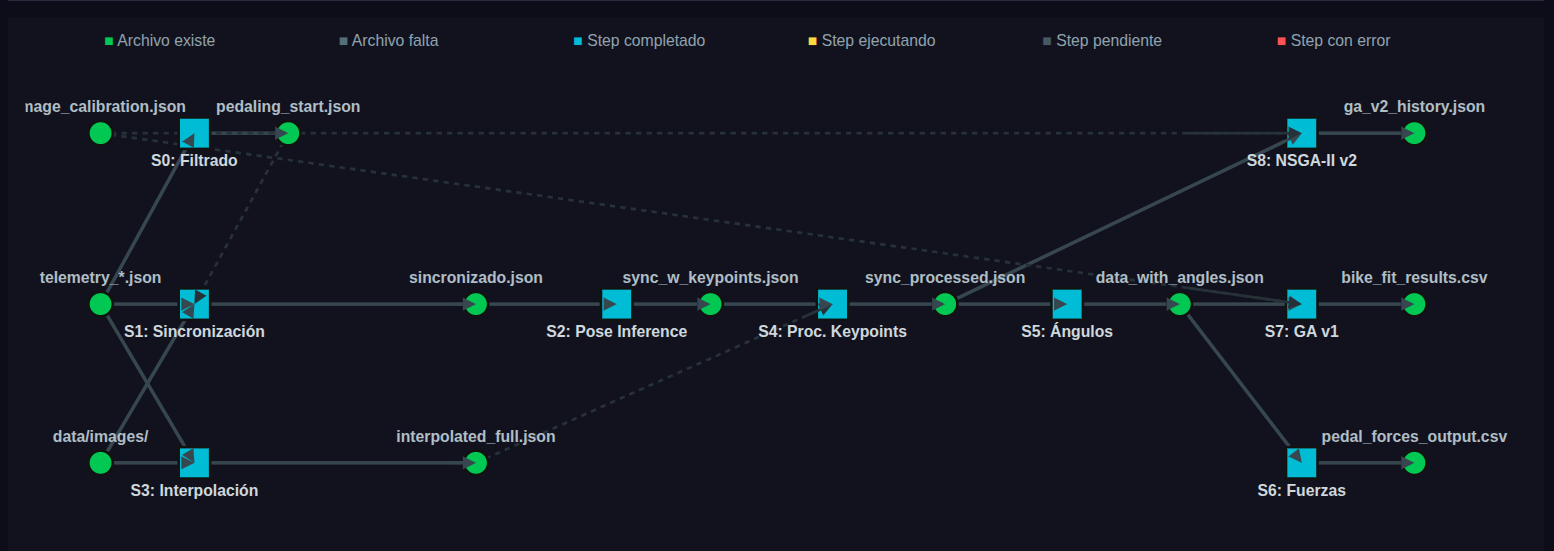
\includegraphics[width=0.90\textwidth]{./Figures/pipeline_real.png}
      \caption{Diagrama del \textit{pipeline} de procesamiento y optimización.
            Se muestran las distintas etapas de transformación de los datos,
            desde la captura de video y telemetría hasta la obtención de los
            parámetros biomecánicos optimizados.}
      \label{fig:pipeline}
\end{figure}
% --------------------------------------

% =============================================================================
\section{Pasos previos al \textit{pipeline}}
\label{sec:pasos_previos}
% =============================================================================

Antes de ejecutar el \textit{pipeline} principal, se realizaron dos pasos de
preparación sobre los datos crudos: la calibración métrica de la cámara y la
selección del inicio efectivo del pedaleo. Ambos pasos se describen a
continuación.

% -----------------------------------------------------------------------------
\subsection{Calibración métrica de la cámara}
\label{ssec:calibracion}
% -----------------------------------------------------------------------------

Para establecer la correspondencia entre el espacio de píxeles de la imagen y
el espacio métrico real, se determinó la relación de píxeles por milímetro
mediante el \textit{script} \texttt{calibrate\_image.py}. Se utilizó como
referencia la rueda de la bicicleta, cuyo diámetro nominal es de 622~mm
(estándar 700c). En la figura~\ref{fig:calibracion} se ilustra el proceso de
calibración: sobre un fotograma representativo se superpone un círculo cuyos
extremos se ajustan manualmente al contorno de la rueda, con lo que se obtiene
la relación métrica de la cámara para esa sesión.

% --- Figura: calibración métrica ---
\begin{figure}[H]
      \centering
      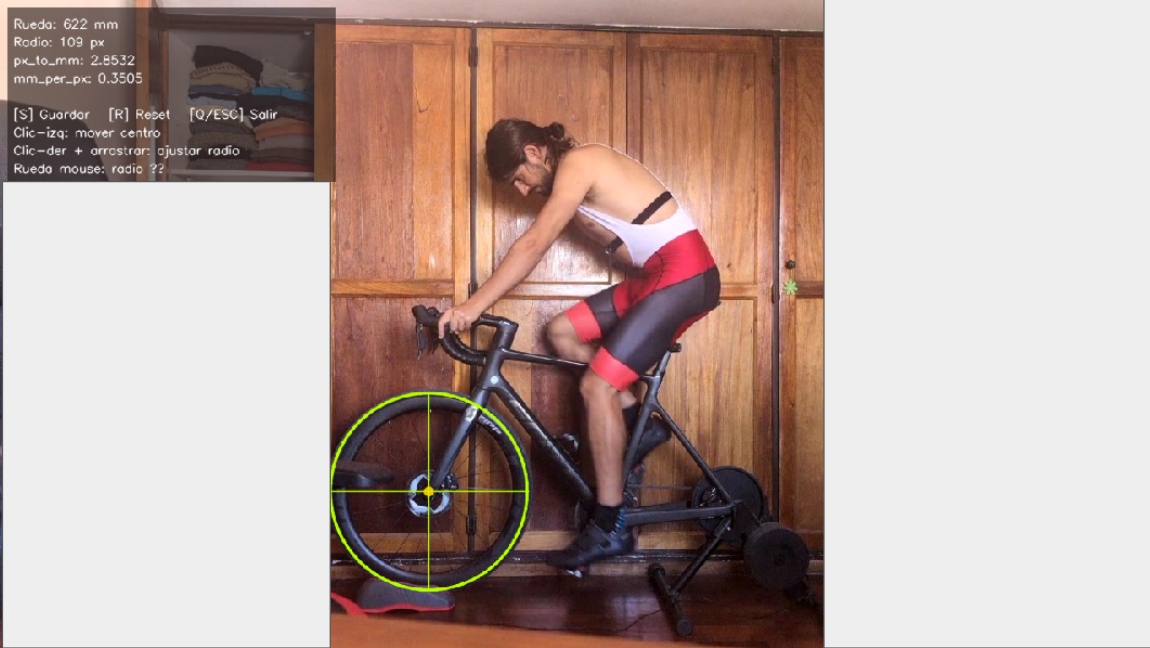
\includegraphics[width=0.80\textwidth]{./Figures/calibracion.png}
      \caption{Interfaz del \textit{script} de calibración métrica. El círculo
            superpuesto al fotograma se ajusta al diámetro de la rueda
            (622~mm, estándar 700c) para obtener la relación de
            píxeles por milímetro.}
      \label{fig:calibracion}
\end{figure}
% ------------------------------------

% -----------------------------------------------------------------------------
\subsection{Selección del inicio del pedaleo}
\label{ssec:seleccion_inicio}
% -----------------------------------------------------------------------------

Con el objeto de excluir los fotogramas previos a la estabilización del ciclo
de pedaleo, se desarrolló el \textit{script} \texttt{filter\_start.py}. Este
\textit{script} analiza la cadencia registrada por el rodillo inteligente e
identifica el primer instante en que dicho valor supera los 80~RPM de forma
sostenida. A partir de ese fotograma se conservan los datos de video y
telemetría; los registros anteriores son descartados. En la
figura~\ref{fig:seleccion_inicio} se muestra la interfaz del \textit{script},
donde la gráfica superior presenta la evolución de la cadencia y la línea
vertical indica el punto de inicio seleccionado.

% --- Figura: selección del inicio ---
\begin{figure}[H]
      \centering
      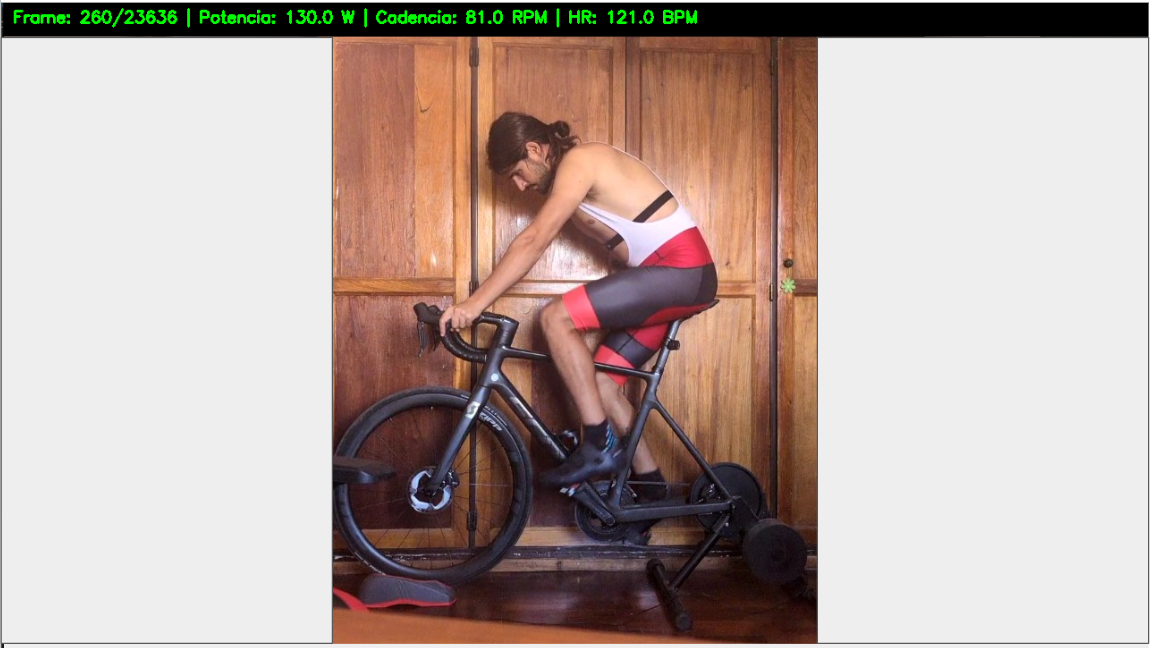
\includegraphics[width=0.80\textwidth]{./Figures/seleccion_inicio.png}
      \caption{Interfaz del \textit{script} \texttt{filter\_start.py}. La
            gráfica superior muestra la cadencia registrada durante la sesión;
            la línea vertical indica el fotograma de inicio seleccionado,
            correspondiente al instante en que la cadencia supera los
            80~RPM de forma sostenida.}
      \label{fig:seleccion_inicio}
\end{figure}
% ------------------------------------